% Left: the 12th roots of unity, primitive ones highlighted. Right: the six chords from 1 in the regular heptagon. Generated by a short script.
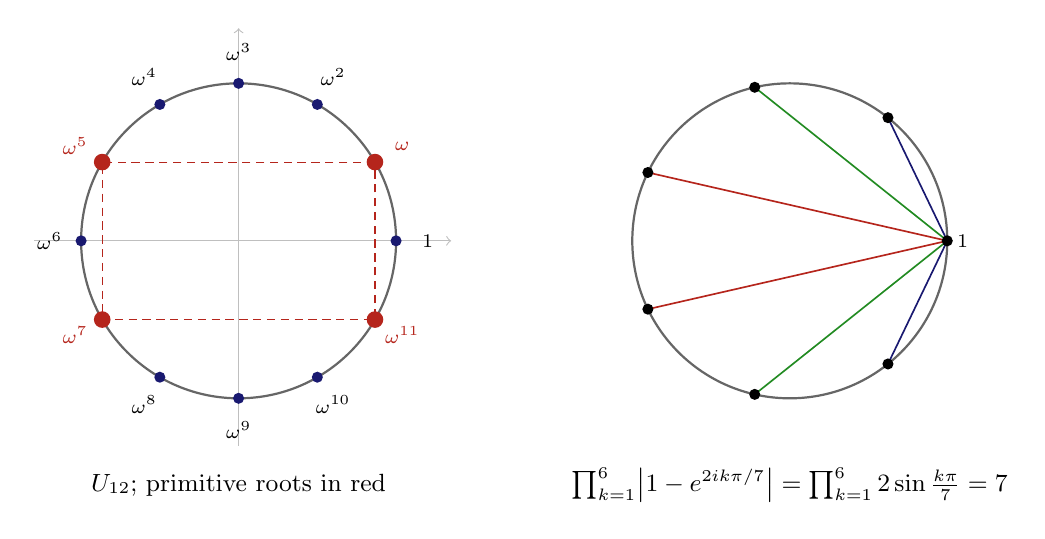
\begin{tikzpicture}
\begin{scope}
\draw[gray!50,->] (-2.6,0)--(2.7,0); \draw[gray!50,->] (0,-2.6)--(0,2.7);
\draw[thick,black!60] (0,0) circle (2);
\fill[MidnightBlue] (2.000,0.000) circle (2pt);
\node[font=\scriptsize,black] at (2.400,0.000) {$1$};
\fill[BrickRed] (1.732,1.000) circle (3pt);
\node[font=\scriptsize,BrickRed] at (2.078,1.200) {$\omega$};
\fill[MidnightBlue] (1.000,1.732) circle (2pt);
\node[font=\scriptsize,black] at (1.200,2.078) {$\omega^{2}$};
\fill[MidnightBlue] (0.000,2.000) circle (2pt);
\node[font=\scriptsize,black] at (0.000,2.400) {$\omega^{3}$};
\fill[MidnightBlue] (-1.000,1.732) circle (2pt);
\node[font=\scriptsize,black] at (-1.200,2.078) {$\omega^{4}$};
\fill[BrickRed] (-1.732,1.000) circle (3pt);
\node[font=\scriptsize,BrickRed] at (-2.078,1.200) {$\omega^{5}$};
\fill[MidnightBlue] (-2.000,0.000) circle (2pt);
\node[font=\scriptsize,black] at (-2.400,0.000) {$\omega^{6}$};
\fill[BrickRed] (-1.732,-1.000) circle (3pt);
\node[font=\scriptsize,BrickRed] at (-2.078,-1.200) {$\omega^{7}$};
\fill[MidnightBlue] (-1.000,-1.732) circle (2pt);
\node[font=\scriptsize,black] at (-1.200,-2.078) {$\omega^{8}$};
\fill[MidnightBlue] (-0.000,-2.000) circle (2pt);
\node[font=\scriptsize,black] at (-0.000,-2.400) {$\omega^{9}$};
\fill[MidnightBlue] (1.000,-1.732) circle (2pt);
\node[font=\scriptsize,black] at (1.200,-2.078) {$\omega^{10}$};
\fill[BrickRed] (1.732,-1.000) circle (3pt);
\node[font=\scriptsize,BrickRed] at (2.078,-1.200) {$\omega^{11}$};
\draw[BrickRed,densely dashed] (1.732,1.000)--(-1.732,1.000)--(-1.732,-1.000)--(1.732,-1.000)--cycle;
\node[font=\small] at (0,-3.1) {$\mathbb U_{12}$; primitive roots in red};
\end{scope}
\begin{scope}[xshift=7cm]
\draw[thick,black!60] (0,0) circle (2);
\draw[MidnightBlue,semithick] (2,0)--(1.247,1.564);
\draw[ForestGreen,semithick] (2,0)--(-0.445,1.950);
\draw[BrickRed,semithick] (2,0)--(-1.802,0.868);
\draw[BrickRed,semithick] (2,0)--(-1.802,-0.868);
\draw[ForestGreen,semithick] (2,0)--(-0.445,-1.950);
\draw[MidnightBlue,semithick] (2,0)--(1.247,-1.564);
\fill (2.000,0.000) circle (2pt);
\fill (1.247,1.564) circle (2pt);
\fill (-0.445,1.950) circle (2pt);
\fill (-1.802,0.868) circle (2pt);
\fill (-1.802,-0.868) circle (2pt);
\fill (-0.445,-1.950) circle (2pt);
\fill (1.247,-1.564) circle (2pt);
\node[font=\scriptsize,right] at (2,0) {$1$};
\node[font=\small,align=center] at (0,-3.1) {$\prod_{k=1}^{6}\bigl|1-e^{2ik\pi/7}\bigr|=\prod_{k=1}^{6}2\sin\frac{k\pi}7=7$};
\end{scope}
\end{tikzpicture}
